\chapter{Ανάλυση Απαιτήσεων Συστήματος}
\label{chap3}

Η εφαρμογή που πραγματεύεται η παρούσα διπλωματική εργασία προορίζεται για χρήση πάνω σε πλατφόρμες κινητών συσκευών που είναι συνδεδεμένες σε δίκτυο. Σκοπός της εφαρμογής είναι να βελτιστοποιήσει τη διαδικασία της ενημέρωσης για κοινωνικοπολιτισμικά δρώμενα και να προσφέρει μια ολοκληρωμένη εμπειρία στους χρήστες της. Αυτό σημαίνει ότι ο χρήστης θα μπορεί να δημιουργήσει τον προσωπικό του λογαριασμό και να ενημερώνεται για εκδηλώσεις που λαμβάνουν χώρα αυτή τη στιγμή γύρω του, όποτε το επιθυμεί. Ο χρήστης θα μπορεί να περιηγηθεί στην κεντρική διεπιφάνεια της εφαρμογής με τη βοήθεια μιας διεπαφής χάρτη, να αναρτήσει σχόλια σχετικά με κάποιο γεγονός στην τοποθεσία του και να αλληλεπιδράσει με άλλους χρήστες που βρισκονται στην περιοχή. Η εφαρμογή θα βοηθάει στο συντονισμό όλων των ατόμων που σχετίζονται με την εκδήλωση, είτε αυτοί είναι οι διοργανωτές, είτε είναι οι συμμετέχοντες.

Το παρόν κεφάλαιο καταπιάνεται με την ανάλυση των απαιτήσεων του συστήματος. Θα γίνει μια εκτενής επεξήγηση κάθε λειτουργικότητας της εφαρμογής και θα παρουσιαστούν οι βασικές αρχές που τις διέπουν.

\section{Γενική Περιγραφή}
Η εφαρμογή αποτελείται από τρία μέρη: (α) τον \tl{client}, (β) τον \tl{server} και (γ) τη βάση δεδομέων. Ο \tl{client} είναι η διεπιφάνεια όπου δρα ο χρήστης, ενώ ο \tl{server} αποτελείται από το σύνολο των μεθόδων υπεύθυνων για την εκτέλεση αιτημάτων από τον \tl{client} (βλ. Σχ. \ref{appecosystem}).

Ο \tl{client} αποτελείται από ένα δρομολογητή (\tl{router}) που συνίσταται από τις διεπιφάνειες της εφαρμογής με τις οποίες μπορεί να αλληλεπιδράσει ο χρήστης. Η κεντρική διεπιφάνεια αποτελείται από μια διεπαφή χάρτη (\tl{Apple Maps API}) για την προβολή σημείων ενδιαφέροντος, τα οποία από εδώ και στο εξής θα αποκαλούνται \tl{\textit{hotspots}}. Ο \tl{router} απαρτίζεται ακόμη από τις σελίδες \tl{\textit{comments, hotspots, profile, new hotspot}}. Καθεμία από αυτες θα αναλυθεί σε επόμενη ενότητα (βλ. ενότητα 3.3.1). Η υλοποίηση και ο έλεγχος του \tl{client} έγιναν με τη βοήθεια φυσικής συσκευής με λειτουργικό \tl{iOS} 12, καθώς και ειδικού \tl{SDK} για αυτό το σκοπό (περισσότερες λεπτομέρειες θα δωθούν στο Κεφ. \ref{chap6}).

Ο \tl{server} καθορίζει τις λειτουργίες προς εκτέλεση που αντιστοιχούν στις αιτήσεις που δημιουργεί ο χρήστης μέσω του \tl{UI} της εφαρμογής. Οι λειτουργίες αυτές συνοπτικά είναι η αποθήκευση των διαπιστευτηρίων και των προσωπικών πληροφοριών του χρήστη, η δημιουργία λογαριασμού (\tl{profile}), η δημιουργία και επεξεργασία δημοσιεύσεων (\tl{create/update hotspot}), η δημιουργία σχολίων (\tl{create comment}), η λήψη και αποθήκευση φωτογραφιών κλπ. Η κατασκευή του \tl{server} έχει δομή τέτοια ώστε να αποσκοπεί στη συνεργατική δράση του με τον \tl{client}, με αποδοτικό και αποτελεσματικό τρόπο.

Η εφαρμογή θα διαθέτει επίσης μια βάση δεδομέων για την αποθήκευση των χρηστών, των δημοσιεύσεων, των σχολίων και άλλων στοιχείων που αφορούν το χρήστη, είτε άμεσα (στοιχεία λογαριασμού, δημοσιεύσεις χρήστη, σχολιασμοί χρήστη κλπ), είτε έμεσσα (σχόλια σε αναρτήσεις του χρήστη, σχόλια σε δημοσιεύσεις άλλων χρηστών κλπ.).  


\begin{figure}[h]
    \centering
    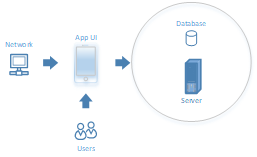
\includegraphics[scale=1]{figures/app-ecosystem.png}
    \caption{Περιβάλλον συστήματος εφαρμογής}
    \label{appecosystem}
\end{figure}

\section{Απαιτήσεις Συστήματος}
Σε αυτή την ενότητα αναφέρονται συνοπτικά οι απαιτήσεις του συστήματος που εξασφαλίζουν την ολοκληρωμένη λειτουργία της εφαρμογής. Πρόκειται για τις λειτουργικότητες της εφαρμογής οι οποίες προσφέρουν την επιθυμητή εμπειρία στο χρήστη. Στο σύνολό τους, οι λειτουργικότητες θα πρέπει να εξυπηρετούν το σκοπό για τον οποίο αναπτύχθηκε η εφαρμογή (βλ. ενότητα 3.2.1). Επίσης, προκειμένου να εξασφαλιστεί η ολοκληρωμένη και καλή εμπειρία του χρήστη, είναι απαραίτητο να ληφθούν υπόψη και κάποιες μη λειτουργικές απαιτήσεις. Οι μη λειτουργικές απαιτήσεις δεν έχουν να κάνουν με την υλοποίηση της διεπιφάνειας του χρήστη, αλλά με τη γενικότερη λειτουργικότητα της εφαρμογής. Η ανάλυση αυτών γίνεται στην ενότητα 3.2.2.

\subsection{Λειτουργικές Απαιτήσεις Συστήματος}
Η διεπιφάνεια του χρήστη θα πρέπει να φέρει τις παρακάτω λειτουργικότητες:

\begin{enumerate}
    \item \textbf{Εγγραφή χρήστη} \\
    Ο χρήστης μπορεί να πραγματοποιήσει εγγραφή στην εφαρμογή, με τη συμπλήρωση κατάλληλης φόρμας.
    \item \textbf{Σύνδεση χρήστη} \\
    Υπάρχοντες χρήστες μπορούν να πραγματοποιήσει σύνδεση στην εφαρμογή, μέσω της συμπλήρωσης κατάλληλης φόρμας με τα διαπιστευτήριά του.
    \item \textbf{Ταυτοποίηση χρήστη} \\
    Η ταυτότητα του χρήστη πιστοποιείται μέσω της έκδοσης \tl{token} με το \tl{OAuth} πρωτόκολλο.
    \item \textbf{Δημοσίευση κατάστασης -- \tl{\textit{hotspot}}} \\
    Ο χρήστης μπορεί να αναρτήσει μια δημοσίευση, σχετική με κάποιο εγγύς γεγονός ή εκδήλωση. Η ανάρτηση θα εμφανίζεται στην διεπιφάνεια χάρτη της κεντρικής σελίδας, στην τοποθεσία του χρήστη. Κατα τη δημιουργία \tl{hotspot} είναι εφικτές οι ακόλουθες επιλογές:
    \begin{itemize}
        \item προσθήκη περιγραφής (απαιτείται)
        \item προσθήκη φωτογραγίας (προεραιτικά)
        \item προσδιορισμός διάρκειας ισχύος της δημοσίευσης (απαιτείται)
    \end{itemize}
    \item \textbf{Ανάγνωση \tl{hotspot} άλλων χρηστών} \\
    Ο χρήστης μπορεί να «ανοίξει» και να διαβάσει \tl{hotspots} άλλων χρηστών στην περιοχή του ή σε άλλη περιοχή, μετακινόντας το χάρτη.
    \item \textbf{Δημιουργία Σχολίων} \\
    Ο χρήστης μπορεί να σχολιάσει σε όλα τα \tl{hotspots} (δικά του και άλλων χρηστών).
    \item \textbf{Προβολή προσωπικών \tl{hotspots}} \\
    Ο χρήστης μπορεί να επισκεφτεί τη λίστα με όλα τα προσωπικά του \tl{hotspots}. Η λίστα είναι ταξινομημένη με το πιο πρόσφατο \tl{hotspot} να φαίνεται πρώτο και το παλαιότερο \tl{hotspot} να φαίνεται τελευταίο.
    \item \textbf{Προβολή πρόσθετων πληροφοριών \tl{hotspot}} \\
    Ο χρήστης μπορεί να επιβλέπει την κατάσταση όλων των \tl{hotspots} (δικών του και άλλων χρηστών) μέσω δεικτών μέτρησης \tl{views} και \tl{comments}. Ο δείκτης \tl{views} είναι υπεύθυνος για τον αριθμό νέων αναγνώσεων ενός \tl{hotspot}, ενώ ο δείκτης \tl{comments} δείχνει τον αριθμό των σχολίων ενός \tl{hotspot}. 
    \item \textbf{Επιλογή φίλτρου αναζήτησης} \\
    Ο χρήστης μπορεί να επιλέξει μια κατηγορία ενδιαφέροντος και να πραγματοποιήσει αναζήτηση στον χάρτη σημείων που ανήκουν σε αυτή. Με το σύρσιμο της οθόνης νέα σημεία εμφανίζονται στο χάρτη.
    \item \textbf{Αναίρεση φίλτρου αναζήτησης} \\
    Ο χρήστης μπορεί να καταργήσει τα επιλεγμένο φίλτρο για να επιλέξει νέο, ή να «καθαρίσει» το χάρτη.
    \item \textbf{Μπάρα Αναζήτησης} \\
    Ο χρήστης μπορεί να πληκτρολογήσει κάποιο σημείο ενδιαφέροντος (\tl{point of interest}) και να πραγματοποιήσει συγκεκριμένη αναζήτηση του επιλεγμένου σημείου. 
    \item \textbf{Άνοιγμα κεντρικού μενού πλοήγησης} \\
    Ο χρήστης μπορεί να πατήσει στο κεντρικό μενού (\tl{\textit{FAB}}) και να επιλέξει τη σελίδα στην οποία θέλει να μεταβεί. Ο χρήστης μπορεί να πλοηγηθεί στις παρακάτω σελίδες:
    \begin{itemize}
        \item λίστα προσωπικών \tl{hotspots}
        \item φόρμα δημοσίευσης νέου \tl{hotspot}
        \item προσωπικό λογαριασμό (\tl{profile}) χρήστη
    \end{itemize}
    \item \textbf{Προβολή προσωπικών στοιχείων} \\
    Ο χρήστης μπορεί να μεταβεί στο \tl{profile} του και να δει τα προσωπικά του στοιχεία.
    \item \textbf{Επεξεργασία προσωπικών στοιχείων} \\
    Ο χρήστης μπορεί να επεξεργαστεί τα προσωπικά του στοιχεία και να ανανεώσει το προσωπικό του λογαριασμό μέσω κατάλληλης φόρμας. Μπορεί να ανανεώσει τα διαπιστευτήριά του, την εικόνα \tl{profile}, το όνομά του, τον τόπο διαμονής, την ημερομηνία γέννησης και το γένος.
    \item \textbf{Προβολή στατιστικών μετρήσεων} \\
    Ο χρήστης μπορεί να δει στατιστικά δεδομένα σχετικά με την δράση του στην εφαρμογή, όπως αριθμό \tl{hotspots}, αριθμό σχολίων, αριθμό ατόμων που επισκέφτηκαν τα \tl{hotspots} του χρήστη, ποσοστό αγοριών/κοριτσιών, δημοτικότητα κλπ. 
    \item \textbf{Αποσύνδεση} \\
    Ο χρήστης μπορεί να αποσυνδεθεί από το λογαριασμό του κάνοντας \tl{logout} (από τη σελίδα του \tl{profile} του).
\end{enumerate}



\subsection{Μη Λειτουργικές Απαιτήσεις Συστήματος}
Η εφαρμογή θα πληροί και ορισμένες μη λειτουργικές απαιτήσεις για μια ολοκληρωμένη εμπειρία χρήστη. Οι απαιτήσεις αυτές απαριθμούνται στη συνέχεια.

\begin{enumerate}
    \item \textbf{Απόδοση -- \tl{Performance}} \\
    Ο χρόνος απόκρισης του συστήματος σην εξυπηρέτηση αιτημάτων από το \tl{server} θα πρέπει να είναι μικρός. Το σύστημα θα πρέπει να μπορεί να ανταποκρίθεί σε μεγάλο αριθμό αιτημάτων.
    \item \textbf{Ταχύτητα ανάκτησης -- \tl{Recoverability}} \\
    Το σύστημα θα πρέπει να μπορεί να ανακτήσει την επιθυμητή κατάσταση λειτουργίας γρήγορα, σε περίπτωση αποτυχίας ή απότομου τερματισμού.
    \item \textbf{Υποστήριξη -- \tl{Documentation}} \\
    Η εφαρμογή θα πρέπει να συνοδεύεται από έγγραφη τεκμηρίωση. Η τεκμιρίωση θα πρέπει να είναι επεξηγηματική και εκτενής προκειμένου να καλύπτει όλα τα πιθανά ζητήματα που μπορεί να προκύψουν.
    \item \textbf{Ασφάλεια -- \tl{Security}} \\
    Η εφαρμογή θα πρέπει να εξασφαλίζει την ασφάλεια των προσωπικών δεδομένων των χρηστών της. Ευαίσθητα δεδομένα όπως κωδικοί ασφαλείας θα πρέπει να κρυπτογραφούνται πριν την αποθήκευσή τους στη βάση, για την αποφυγή κατάχρησης από κακόβουλους χρήστες.
    \item \textbf{Επεκτασιμότητα -- \tl{Extensibility/Scalability}} \\
    Η υλοποίηση της εφαρμογής θα πρέπει να στηρίζεται σε τεχνολογίες που επιτρέπουν την μελλοντική επέκτασή της με νέα χαρακτηριστικά και πρόσθετες εφαρμογές. Επιπλέον, η εφαρμογή θα πρέπει να μπορεί να διαχειριστεί μεγάλο αριθμό χρηστών.
\end{enumerate}



\section{Αρχιτεκτονική Εφαρμογής}
%Σε 2-3 παραγράφους εξηγούμε ότι θα ακολουθήσει η ανάλυση του προβλήματος που πραγματεύεται η διπλωματική.
Όπως είδαμε στο  σχ. \ref{appecosystem}, το περιβάλλον της εφαρμογής διαμορφώνεται από τρεις βασικούς συντελεστές: τον \tl{client}, τον \tl{server} και τη βάση δεδομένων. Ο \tl{client} θα πρέπει να είναι συνδεδεμένος σε δίκτυο προκειμένου να εδραιωθεί η επικοινωνία με τον \tl{server}. Ο \tl{server} της εφαρμογής φιλοξενείται από έναν κεντρικό εξυπηρετητή μέσω μιας διαδικασίας γνωστής ως \tl{hosting}. [υλοποιώ και επανέρχομαι να πω περισσότερα]. Η διεπικοινωνία μεταξύ \tl{client-server} είναι υπεύθυνη για την σωστή λειτουγία της εφαρμογής και την διασφάλιση μιας ολοκληρωμένης εμπειρίας από την πλευρά του χρήστη. 

Ο \tl{client} είναι υπεύθυνος για την διαμόρφωση ενός διaδραστικού περιβάλλοντος για τον χρήστη. Το περιβάλλον αυτό αποτελείται από έναν \tl{router} ο οποίος είναι υπεύθυνος για την πλοήγηση του χρήστη στις διάφορες σελίδες της εφαρμογής. Σε κάθε σελίδα, υπάρχουν διαδραστικά στοιχεία όπως γραφικές διεπιφάνειες, διεπαφές, πλήκτρα ενεργειών και στοιχεία εισόδου και διάφορα άλλα στοιχεία αλληλεπίδρασης, όλα με σκοπό την παροχή μιας πλήρους εμπειρίας στο χρήστη.

Ο \tl{server} αναλαμβάνει να εξυπηρετήσει τα αιτήματα που δημιουργεί ο χρήστης από την πλευρά του \tl{client}. Κάθε φορά που ο χρήστης πραγματοποιεί μια ενέργεια που απαιτεί δεδομένα από τον \tl{server}, τότε δημιουργείται ένα αίτημα το οποίο καλείται να εξυπηρετήσει ο \tl{server}. Η προβολή κάποιου \tl{hotspot}, η δημιουργία ενός σχολίου, η επεξεργασία του λογαριασμού του χρήστη, αποτελούν μερικά παραδείγματα τέτοιων αιτημάτων.

Η βάση δεδομένων αποτελεί τον αποθηκευτικό χώρο της εφαρμογής. Όλα τα δεδομένα, από το λογαριασμό του χρήστη μέχρι και τον αριθμό προβολών ενός \tl{hotspot}, αποθηκεύονται σε συλλογές εντός της βάσης. Έτσι, κάθε φορά που ζητούνται δεδομένα, ο \tl{server} πραγματοποιεί αναζήτηση κατάλληλης μορφής στη βάση και επιστρέφει τα απαραίτητα δεδομένα στον \tl{client}.


\subsection{Υποδομή \tl{Client} και Σενάρια Χρήσης (\textit{\tl{Frontend}})}
Στις επόμενες ενότητες ακολοθεί μια επεξηγηματική ανάλυση της αρχιτεκτονικής του παραπάνω συστήματος. Θα παρουσιαστούν οι υποδομές της εφαρμογής και οι οθόνες που τις θεμελιώνουν. Έπειτα, θα αναλυθούν όλα τα πιθανά σενάρια χρήσης (\tl{use cases}) της εφαρμογής. 

\subsubsection{Οθόνες Εφαρμογής}
Η εφαρμογή δομείται σε τέσσερα κύρια μέρη: ταυτοποίηση, κεντρική σελίδα χάρτη, \tl{hotspots} και \tl{profile}. Οι αντίστοιχες οθόνες (\tl{screens}) αυτών είναι:
\item (α) οθόνη έναρξης (\textit{\tl{WelcomeScreen}})

Εκεί μεταφέρεται ο χρήστης την πρώτη φορά που ανοίγει την εφαρμογή, ή όταν αποσυνδεθεί από το λογαριασμό του.

\item (β) οθόνη ταυτοποίσης χρήστη (\textit{\tl{SignUpScreen \& LoginScreen}}) 

Η οθόνη ταυτοποίησης χρήστη αποτελείται από δυο \tl{tabs} (\tl{Register, Login}), καθένας εκ των οποίων περιέχει φόρμα κατάλληλης μορφής την οποία καλείται να συμπληρώσει ο χρήστης.

\item (γ) κεντρική οθόνη χάρτη (\textit{\tl{HomeScreen}})

Η κεντρική οθόνη αποτελείται κυρίως από τη διεπαφή χάρτη (\tl{Apple Map API}). Στον χάρτη φαίνονται όλα τα \tl{hotspots} και ο χρήστης μπορεί να ανανεώνει το περιεχόμενο, αλλάζοντας τη θέση του χάρτη.

\item (ε) οθόνη δημιουργίας νέου \tl{hotspot} (\textit{\tl{CreateHotspotScreen}})

Η οθόνη αυτή συνίσταται από μια φόρμα όπου ο χρήστης εισάγει τα στοιχεία του \tl{hotspot} προς δημιουργία.

\item (δ) οθόνη επεξεργασίας \tl{hotspot} (\textit{\tl{EditHotspotScreen}})

Εάν ο χρήστης το επιθυμεί, μπορεί να επεξεργαστεί ένα από τα δικά του \tl{hotspots} εδώ.

\item (στ) οθόνη προσωπικών \tl{hotspot} (\textit{\tl{HotspotListScreen}})

Εδώ μπορεί να πλοηγηθεί ο χρήστης όταν επιθυμεί να προβάλλει όλα τα \tl{hotspots} που έχει δημιουργήσει ο ίδιος.  

\item (ζ) οθόνη προσωπικού \tl{profile} (\textit{\tl{ProfileScreen}})

Σε αυτή την οθόνη, ο χρήστης μπορεί να προβάλλει τα στοιχεία του λογαριασμού του.

\item (η) οθόνη επεξεργασίας \tl{profile} (\textit{\tl{EditProfileScreen}})

Εάν ο χρήστης επιθυμεί να αλλάξει τα στοιχεία του προσωπικού του λογαριασμού ή να επεξεργαστεί κάποια από αυτά, μπορεί να το κάνει σε αυτή τη σελίδα. Η οθόνη αποτελείται από μια φόρμα η οποία περιέχει τα αρχικά στοιχεία του χρήστη πριν από την αλλαγή. Για την ολοκλήρωση της διαδικασίας απαιτείται ο κωδικός του χρήστη για επιβεβαίωση. 

\item (θ) οθόνη στατιστικών δεδομένων (\textit{\tl{StatisticsScreen}})

Στατιστικά δεδομένα σχετικά με τη χρήση της εφαρμογής και την αλληλεπίδραση με άλλους χρήστες εμφανίζονται στην οθόνη στατιστικών δεδομένων.


\subsubsection{Σενάρια Χρήσης Εφαρμογής}

\paragraph{Εγγραφή Χρήστη στην Εφαρμογή (\textit{\tl{Register}})}
\begin{enumerate}
    \item Ο χρήστης ανοίγει την εφαρμογή και πατάει το πλήκτρο ``\textit{\tl{Get Started}}'' στην οθόνη έναρξης (\textit{\tl{WelcomeScreen}}).
    \item Ο χρήστης συμπλήρώνει τη φόρμα εγγραφής που βρίσκεται στο \tl{tab} με την ονομασία \tl{register}. Στη φόρμα ο χρήστης πρέπει να εισάγει όλες τις απαιτούμενες πληροφορίες. Τα απαιτούμενα πεδία είναι τα εξής:
    \begin{itemize}
        \item πλήρες όνομα (\textit{\tl{fullname}})
        \item όνομα χρήστη (\textit{\tl{username}})
        \item ηλεκτρονική διεύθυνση (\textit{\tl{email}})
        \item κωδικός (\textit{\tl{password}})
        \item επαλήθευση κωδικού (\textit{\tl{confirm password}})
        \item ημερομηνία γέννησης (\textit{\tl{birthdate}})
        \item πόλη (\textit{\tl{city}})
        \item γένος χρήστη (\textit{\tl{gender}})
    \end{itemize}
    Εάν ο χρήστης το επιθυμεί, μπορεί να επιλέξει μια φωτογραφία \tl{profile} από τη συλλογή φωτογραφιών του ή να βγάλει καινούρια μέσω της κάμερας της συσκευής.
    \item Στην περίπτωση που δεν υπάρχουν σφάλματα κατά την υποβολή της φόρμας εγγραφής, ο χρήστης εγγράφεται στην εφαρμογή με επιτυχία. Η εφαρμογή τον πηγαίνει αυτόματα στην κεντρική σελίδα της διεπαφής χάρτη (\textit{\tl{HomeScreen}}).
\end{enumerate}

\paragraph{Σύνδεση Χρήστη στην Εφαρμογή (\textit{\tl{Login}})}
\begin{enumerate}
    \item Ο χρήστης ανοίγει την εφαρμογή και πατάει το πλήκτρο ``\textit{\tl{Get Started}}'' στην οθόνη έναρξης (\textit{\tl{WelcomeScreen}}).
    \item Ο χρήστης συμπλήρώνει τη φόρμα σύνδεσης που βρίσκεται στο \tl{tab} με την ονομασία \tl{login}. Στη φόρμα ο χρήστης πρέπει να εισάγει όλες τις απαιτούμενες πληροφορίες. Τα απαιτούμενα πεδία είναι τα εξής:
    \begin{itemize}
        \item ηλεκτρονική διεύθυνση (\textit{\tl{email}})
        \item κωδικός πρόσβασης (\textit{\tl{password}})
    \end{itemize}
    \item Στην περίπτωση που δεν υπάρχουν σφάλματα κατά την υποβολή της φόρμας σύνδεσης, ο χρήστης επαναφέρεται αυτόματα στην αρχική σελίδα (\textit{\tl{HomeScreen}}).
\end{enumerate}

\paragraph{Δημιουργία Νέου \tl{Hotspot}}
\begin{enumerate}
    \item Ο χρήστης πατάει πάνω στο \tl{FAB} στο κάτω δεξία μέρος της οθόνης στην \tl{HomeScreen}.
    \item Ο χρήστης πατάει επάνω στο εικονίδιο με το σύμβολο ``\textit{\tl{plus}}'' από το κεντρικό μενού πλοήγησης που εμφανίζεται.
    \item ο χρήστης μεταφέρεται στη σελίδα δημιουργίας νέου \tl{Hotspot} (\textit{\tl{CreateHotspotScreen}}).
    
    \item Ο χρήστης συμπλήρώνει τη φόρμα δημιουργίας νέου \tl{Hotspot}. Τα απαιτούμενα πεδία είναι τα εξής:
    \begin{itemize}
        \item περιγραφή (\textit{\tl{description}})
        \item χρονική διάρκεια ισχύος σε λεπτά (\textit{\tl{validity}})
        
    \end{itemize}
    Εάν ο χρήστης το επιθυμεί, μπορεί να προσθέσει μια φωτογραφία από τη συλλογή φωτογραφιών του ή να βγάλει καινούρια μέσω της κάμερας της συσκευής.
    \item Στην περίπτωση που δεν υπάρχουν σφάλματα κατά τη δημιουργία νέου \tl{Hotspot}, η διαδικασία ολοκληρώνεται επιτυχώς και ο χρήστης μεταφέρεται αυτόματα στην αρχική σελίδα. Το νέο \tl{Hotspot} θα εμφανίζεται στο χάρτη στην τοποθεσία του χρήστη.
\end{enumerate}

\paragraph{Γρήγορη Προβολή \tl{Hotspot}}
\begin{enumerate}
    \item Στο χάρτη της αρχικής οθόνης, ο χρήστης πατάει πάνω στο εικονίδιο ενός \tl{hotspot} (\textit{\tl{hotspot marker}}).
    \item Οι λεπτομέρειες του \tl{hotspot} εμφανίζονται σε ένα ``\textit{παράθυρο}'' ενσωματωμένο στο χάρτη (\textit{\tl{callout}}). ο χρήστης μπορεί να δει την περιγραφή, τον αριθμό σχολίων και προβολών, και αν υπάρχει, την εικόνα του επιλεγμένου \tl{hotspot}.
\end{enumerate}

\paragraph{Προβολή Λεπτομερειών \tl{Hotspot}}
\begin{enumerate}
    \item Στο χάρτη της αρχικής οθόνης, ο χρήστης πατάει πάνω στο εικονίδιο ενός \tl{hotspot} (\textit{\tl{hotspot marker}}).
    \item Οι λεπτομέρειες του \tl{hotspot} εμφανίζονται σε ένα ``\textit{παράθυρο}'' ενσωματωμένο στο χάρτη (\textit{\tl{callout}}). ο χρήστης μπορεί να δει την περιγραφή, τον αριθμό σχολίων και προβολών, και αν υπάρχει, την εικόνα του επιλεγμένου \tl{hotspot}.
    \item Ο χρήστης πατάει πάνω στο εικονίδιο ``\textit{\tl{comments}}'' και μεταφέρεται αυτόματα στην οθόνη λεπτομερειών του συγκεκριμένου \tl{hotspot}.
\end{enumerate}

\paragraph{Δημιουργία Σχολίου}
\begin{enumerate}
    \item Ο χρήστης πηγαίνει στη σελίδα λεπτομερειών ενός \tl{hotspot} (\textit{\tl{CommentsScreen}}) ακολουθώντας τη διαδικασία που περιγράφεται στην παράγραφο \textit{Προβολή Λεπτομερειών \tl{Hotspot}}.
    \item Ο χρήστης πλοηγείται στο κάτω μέρος της σελίδας.
    
    Αλλιώς,
    \item Ο χρήστης σύρει προς τα αριστερά ένα από τα υπάρχοντα σχόλια και πατάει το εικονίδιο ``\textit{\tl{reply}}''.
    \item Ο χρήστης εισάγει το σχόλιό του στο \textit{\tl{comment box}} με επιγραφή ``\textit{\tl{Add a comment...}}''.
    \item Μόλις ο χρήστης ολοκληρώσει το σχόλιό του, πατάει στο εικονίδιο ``\textit{\tl{send}}''.
    \item Σε περίπτωση που το σχόλιο δεν έχει σφάλματα, η διαδικασία ολοκληρώνεται επιτυχώς και το νέο σχόλιο εμφανίζεται τελευταίο στο τμήμα σχολίων της οθόνης.
\end{enumerate}

\paragraph{Προβολή Περισσότερων Σχολίων}
\begin{enumerate}
    \item Ο χρήστης πηγαίνει στη σελίδα λεπτομερειών ενός \tl{hotspot} (\textit{\tl{CommentsScreen}}) ακολουθώντας τη διαδικασία που περιγράφεται στην παράγραφο \textit{Προβολή Λεπτομερειών \tl{Hotspot}}.
    \item Ο χρήστης πλοηγείται στο κάτω μέρος της σελίδας.
    \item Ο χρήστης πατάει το πλήκτο με επιγραφή ``\tl{\textit{more}}''. Πέντε νέα σχόλια εμφανίζονται στο τμήμα σχολίων της οθόνης.
\end{enumerate}

\paragraph{Συγκεκριμένη Αναζήτηση Σημείου Ενδιαφέροντος}
\begin{enumerate}
    \item Στη σελίδα χάρτη (\textit{\tl{HomeScreen}}) ο χρήστης πατάει εντός της μπάρας αναζήτησης με επιγραφή ``\tl{\textit{Search a hotspot...}}'' που βρίσκεται στο πάνω μέρος της οθόνης.
    \item Ο χρήστης πληκτρολογεί το όνομα ή κάποια άλλη λέξι-κλειδί που σχετίζεται με το σημείο ενδιαφέροντος.
    \item Ο χρήστης πατάει σε μία από τις προτεινόμενες επιλογές από τη λίστα που εμφανίζεται.
    \item Το επιλεγμένο σημείο ενδιαφέροντος εμφανίζεται στο χάρτη.
\end{enumerate}

\paragraph{Γενικευμένη Αναζήτηση Σημείου Ενδιαφέροντος}
\begin{enumerate}
    \item Στη σελίδα χάρτη (\textit{\tl{HomeScreen}}) ο χρήστης πατάει εντός της μπάρας αναζήτησης με επιγραφή ``\tl{\textit{Search a hotspot...}}'' που βρίσκεται στο πάνω μέρος της οθόνης.
    \item Ο χρήστης πληκτρολογεί το όνομα ή κάποια άλλη λέξι-κλειδί που σχετίζεται με το σημείο ενδιαφέροντος.
    \item Ο χρήστης πατάει το εικονίδιο ``\tl{\textit{search}}''.
    \item Τα αποτελέσματα εμφανίζονται στο χάρτη.
\end{enumerate}

\paragraph{Αναζήτηση Σημείου Ενδιαφέροντος με Φίλτρο}
\begin{enumerate}
    \item Στη σελίδα χάρτη (\textit{\tl{HomeScreen}}) ο χρήστης πατάει το εικονίδιο ``\tl{\textit{menu}}'' που βρίσκεται στο πάνω αριστερά μέρος της οθόνης.
    \item Στο ``\tl{\textit{drawer menu}}'' που εμφανίζεται, ο χρήστης επιλέγει μία από τις κατηγορίες πατώντας επάνω σε αυτή. Οι διαθέσιμες κατηγορίες είναι:
    \begin{itemize}
        \item \tl{\textit{Coffee}}
        \item \tl{\textit{Food}}
        \item \tl{\textit{Drinks}}
        \item \tl{\textit{Sights}}
        \item \tl{\textit{Arts}}
    \end{itemize}
    \item Τα αποτελέσματα εμφανίζονται στο χάρτη. Κάθε φορά που ο χρήστης αλλάζει τη θέση του χάρτη, νέα αποτελέσματα φορτώνονται στη νέα θέση.
\end{enumerate}

\paragraph{Αναίρεση Αναζήτησης}
\begin{enumerate}
    \item Στη σελίδα χάρτη (\textit{\tl{HomeScreen}}) ο χρήστης πατάει το εικονίδιο ``\tl{\textit{menu}}'' που βρίσκεται στο πάνω αριστερά μέρος της οθόνης.
    \item Στο ``\tl{\textit{drawer menu}}'' που εμφανίζεται, ο χρήστης πατάει την επιλογή ``\tl{\textit{Clear}}''.
    \item Τα αποτελέσματα αφαιρούνται από το χάρτη.
\end{enumerate}

\paragraph{Επαναφορά Θέσης Χάρτη (\textit{\tl{Find My Location}})}
\begin{enumerate}
    \item Στη σελίδα χάρτη (\textit{\tl{HomeScreen}}) ο χρήστης πατάει το εικονίδιο ``\tl{\textit{location}}'' που βρίσκεται στο κάτω αριστερά μέρος της οθόνης.
    \item Η θέση του χάρτη επαναφέρεται στην τοποθεσία του χρήστη.
\end{enumerate}

\paragraph{Προβολή Λίστας Προσωπικών \tl{Hotspots}}
\begin{enumerate}
    \item Ο χρήστης πατάει πάνω στο \tl{FAB} στο κάτω δεξία μέρος της οθόνης στην \tl{HomeScreen}.
    \item Ο χρήστης πατάει επάνω στο εικονίδιο με το σύμβολο ``\textit{\tl{hotspots}}'' από το κεντρικό μενού πλοήγησης που εμφανίζεται.
    \item ο χρήστης μεταφέρεται στη σελίδα προσωπικών \tl{Hotspots} (\textit{\tl{HotspotListScreen}}). Στη λίστα εμφανίζονται λεπτομέρειες των \tl{hotspots} του χρήστη. Ο χρήστης μπορεί να δει την περιγραφή, τον αριθμό σχολίων και προβολών του \tl{hotspot}.
\end{enumerate}

\paragraph{Επεξεργασία Προσωπικού \tl{Hotspot}}
\begin{enumerate}
    \item ο χρήστης μεταφέρεται στη σελίδα προσωπικών \tl{Hotspots} (\textit{\tl{HotspotListScreen}}) ακολουθώντας τη διαδικασία που περιγράφεται στην παράγραφο \textit{Προβολή Λίστας Προσωπικών \tl{Hotspots}}.
    \item Ο χρήστης σύρει προς τα δεξιά το \tl{hotspot} που θέλει να επεξεργαστεί. Στη συνέχεια πατάει στο εικονίδιο ``\textit{\tl{edit}}'' που εμφανίζεται εντός του κίτρινου πλαισίου.
    \item Ο χρήστης μεταφέρεται αυτόματα στη σελίδα επεξεργασίας \tl{hotspot} (\textit{\tl{EditHotspotScreen}}).
    \item Ο χρήστης επεξεργάζεται τα επιθυμητά στοιχεία του \tl{hotspot} και όταν τελειώσει πατάει ``\textit{\tl{Save}}'' στο πάνω δεξιά μέρος της οθόνης.
    \item Σε περίπτωση που δεν υπάρχουν σφάλματα, η διαδικασία ολοκληρώνεται επιτυχώς και οι αλλαγές αποθηκεύονται. Το \tl{hotspot} εμφανίζεται πλέον με τις νέες αλλαγές.
    
\end{enumerate}

\paragraph{Διαγραφή Προσωπικού \tl{Hotspot}}
\begin{enumerate}
    \item ο χρήστης μεταφέρεται στη σελίδα προσωπικών \tl{Hotspots} (\textit{\tl{HotspotListScreen}}) ακολουθώντας τη διαδικασία που περιγράφεται στην παράγραφο \textit{Προβολή Λίστας Προσωπικών \tl{Hotspots}}.
    \item Ο χρήστης σύρει προς τα αριστερά το \tl{hotspot} που θέλει να διαγράψει. Στη συνέχεια πατάει στο εικονίδιο ``\textit{\tl{delete}}'' που εμφανίζεται εντός του κόκκινου πλαισίου.
    \item Το \tl{hotspot} διαγάφεται από τη λίστα προσωπικών \tl{hotspots}.
\end{enumerate}

\paragraph{Προβολή Προσωπικού Λογαριασμού (\textit{\tl{Profile}})}
\begin{enumerate}
     \item Ο χρήστης πατάει πάνω στο \tl{FAB} στο κάτω δεξία μέρος της οθόνης στην \tl{HomeScreen}.
    \item Ο χρήστης πατάει επάνω στο εικονίδιο με το σύμβολο ``\textit{\tl{account}}'' (ή την εικόνα \tl{profile}, αν έχει επιλέξει μία) από το κεντρικό μενού πλοήγησης που εμφανίζεται.
    \item ο χρήστης μεταφέρεται στη σελίδα προσωπικού λογαριασμού (\textit{\tl{ProfileScreen}}). Σε αυτή την οθόνη ο χρήστης μπορεί να προβάλλει τα προσωπικά του στοιχεία.
\end{enumerate}

\paragraph{Επεξεργασία Προσωπικού Λογαριασμού (\tl{\textit{Profile}})}
\begin{enumerate}
     \item ο χρήστης μεταφέρεται στη σελίδα προσωπικού λογαριασμού (\textit{\tl{ProfileScreen}}) ακολουθώντας τη διαδικασία που περιγράφεται στην παράγραφο ``\textit{Προβολή Προσωπικού Λογαριασμού}''.
    \item ο χρήστης πατάει στο πλήκτρο ``\textit{\tl{Edit}}'' που βρίσκεται στο επάνω δεξιά μέρος της οθόνης.
    \item ο χρήστης μεταφέρεται στη σελίδα επεξεργασίας του προσωπικού λογαριασμού (\textit{\tl{EditProfileScreen}}). Η οθόνη αυτή αποτελείται από μια φόρμα με τα αρχικά στοιχεία του χρήστη. Ο χρήστης μπορεί να επεξεργαστεί τα προσωπικα του στοιχεία.
    \item Σε περίπτωση επιτυχούς υποβολής της φόρμας επεξεργασίας των στοιχείων του προσωπικού λογαριασμού, τα νέα στοιχεία αποθηκεύονται στο σύστημα και ο χρήστης επαναφέρεται στο \textit{profile} του.
\end{enumerate}

\paragraph{Προβολή Στατιστικών Δεδομένων Λογαριασμού}
\begin{enumerate}
     \item ο χρήστης μεταφέρεται στη σελίδα προσωπικού λογαριασμού (\textit{\tl{ProfileScreen}}) ακολουθώντας τη διαδικασία που περιγράφεται στην παράγραφο ``\textit{Προβολή Προσωπικού Λογαριασμού}''.
    \item ο χρήστης πατάει στο πλήκτρο βέλους με την επιγραφή ``\textit{\tl{Stats for nerds}}'' στο τμήμα ``\textit{\tl{Settings}}''.
    \item Ο χρήστης μεταφέρεται στη σελίδα στατιστικών δεδομένων του προσωπικού του λογαριασμού (\textit{\tl{StatisticsScreen}}). Η οθόνη διαιρείται σε τρία τμήματα: 
    
    (α) \tl{\textit{account stats}}
    
    Στατιστικά δεδομένα που αφορούν τις κινήσεις του χρήστη εντός της εφαρμογής. Τα δεδομένα αυτά είναι ο συνολικός αριθμός των \tl{hotspots} του χρήστη, o συνολικός αριθμός σχολίων του χρήστη και ο συνολικός αιρθμός προβολών των  \tl{hotspots} του χρήστη από άλλους χρήστες.
    
    (β) \tl{\textit{insights}}
    
    Ποσοστιαίες τιμές που αφορούν την δράση και εξέλιξη του χρήστη εντός της εφαρμογής . Οι τιμές αυτές είναι η δημοτικότητα (\tl{popularity}) και η αλληλεπίδραση (\tl{engagement}) του χρήστη.
    
    (γ) \tl{\textit{audience}}
    
    Διάκριση του κοινού του χρήστη με βάση το γένος (θηλυκό ή αρσενικό). 
    
\end{enumerate}





\subsection{Υποδομή \tl{Server} και Βάσης Δεδομένων (\textit{\tl{Backend}})}
Στην προηγούμενη ενότητα, παρουσιάστηκαν οι βασικές λειτουργικότητες που προσφέρει η εφαρμογή στους χρήστες της. Αναλύθηκαν οι υπηρεσίες της εφαρμογής καθώς επίσης και τα σενάρια με τα οποία ο χρήστης μπορεί να αποκτήσει πρόσβαση σε αυτές. Έτσι, όταν ο χρήστης επιθυμεί για παράδειγμα να δημιουργήσει ένα νέο \tl{hotspot}, αρκεί να πλοηγηθεί στην οθόνη δημιουργίας νέου \tl{hotspot}, να συμπληρώσει την αντίστοιχη φόρμα και να την υποβάλλει. Αυτές είναι οι ενέργειες που πρέπει να γίνουν από την πλευρά του \tl{client}. Αυτή η ενότητα ασχολείται με τις ενέργειες που απαιτούνται από την πλευρά του \tl{server} και τον τρόπο με τον οποίο αυτές είναι σχεδιασμένες να αλληλεπιδρούν μεταξύ τους αλλά και με το υπόλοιπο σύστημα.

Είναι προφανής από τα παραπάνω η ανάγκη αποσύμπλεξης των αιτημάτων προς εξυπηρέτηση από το \tl{server}. Κάθε λειτουργία της εφαρμογής χαρακτηρίζεται από ένα σύνολο ενεργειών που πρέπει να εκτελεστούν κάθε φορά προκειμένου να προκληθεί το επιθυμητό αποτέλεσμα. Για παράδειγμα, η δημιουργία ενός \tl{hotspot} πυροδοτεί μια σειρά αιτημάτων προς τον \tl{server} όπως η συσχέτιση του \tl{hotspot} με το δημιουργό του, η αποθήκευση των δεδομένων του \tl{hotspot} στην βάση, η καταγραφή των σχολίων του \tl{hotspot} κλπ. Έτσι, η σχεδίαση θα πρέπει να βρίσκεται σε συμφωνία με τις απαιτήσεις που πρέπει να πληροί το σύστημα. Ανακύπτει λοιπόν το συμπέρασμα πως είναι αδύνατη η σειριακή εξυπηρέτηση όλων των αιτημάτων από τον ίδιο πόρο, καθώς αυτό θα καθιστούσε το σύστημα υπερβολικά αργό και περίπλοκο.

Συνεπώς, η πρακτική που ακολουθεί η δομή του \tl{server} αποσκοπεί στην αποσυσχέτιση διαφορετικών αιτημάτων. Αυτό επιτυγχάνεται με την ιεράρχηση των λειτουργιών που αφορούν τα αιτήματα, με βάση τη φύση τους. Αιτήματα που σχετίζονται με τους χρήστες θα ανατίθενται αποκλειστικά σε εξυπηρετητές ενεργειών των χρηστών, αιτήματα που αφορούν τα \tl{hotspots} θα ανατίθενται αποκλειστικά σε εξυπηρετητές ενεργειών των \tl{hotspots} κοκ. Η αποθήκευση δεδομέων στη βάση βρίσκεται σε συνοχή με την παραπάνω τακτική, αφού τα δεδομένα μοντελοποιούνται σε \tl{collections} βάσει της φύση τους.  Με αυτό τον τρόπο, επιτυγχάνεται η παραλληλοποίηση των λειτουργιών του \tl{server}, η διαίρεση του φορτίου και η διακριτοποίηση των μεθόδων. Το τελευταίο έχει σημαντική συνεισφορά στην διευκόλυνση της σχεδίασης του συστήματος από τον προγραμματιστή, χάρις τον μεγάλο βαθμό επαναληψιμότητας των περισσότερων τμημάτων. 


\subsection{Διεπικοινωνία Μεταξύ Υποδομών}
Το σύστημα \tl{client-server} επικοινωνεί μέσω αιτημάτων συγκεκριμένου σκοπού. Κάθε φορά που ο χρήστης πραγματοποιεί μια ενέργεια εντός της εφαρμογής, ο \tl{client} δημιουργεί ένα αίτημα προς στον \tl{server}. Το αίτημα αυτό δρομολογείται στον κατάλληλο εξυπηρετητή από την πλευρά του \tl{server}. Έπειτα, ακολουθεί η ανάθεση του αιτήματος στον αντίστοιχο πόρο και η εκτέλεση των απαραίτητων λειτουργιών. Το αποτέλεσμα επηρεάζει τα δεδομένα στη βάση και επιστρέφει με κατάλληλη μορφή πίσω στον \tl{client}. Η παραπάνω διαδικασία γίνεται βέλτιστα, μέσω ασύγχρονων μεθόδων διαχείρισης δεδομένων από και προς τη βάση δεδομένων. Η διαδικασία εξυπηρέτησης αιτημάτων είναι παραλληλοποιημένη ώστε πολλά αιτήματα να εξηπηρετούνται από διαφορετικούς πόρους του συστήματος ταυτόχρονα.

















